\documentclass{scrartcl}

\usepackage{amsmath}
\usepackage{slashed}
\usepackage{amssymb}
\usepackage{amsthm}
\usepackage{mathtools}
\usepackage{stmaryrd}
\usepackage{bussproofs}
\usepackage{listings}
\usepackage{parcolumns}
\usepackage{tikz}
\usepackage{tcolorbox}

\tcbuselibrary{theorems}

\usetikzlibrary{matrix}

	\tikzset{
		table nodes/.style={
			rectangle,
			draw=black,
			align=center,
			minimum height=7mm,
			text depth=0.5ex,
			text height=2ex,
			inner xsep=0pt,
			outer sep=0pt
		},
		table/.style={
			matrix of nodes,
			row sep=\pgflinewidth,
			column sep=\pgflinewidth,
			nodes={
				table nodes
			},
			execute at empty cell={\node[draw=none]{};}
		}
	}

%-- theorem --
%\newtheoremstyle{mydefstyle}{0.5cm}{0.5cm}{}{1cm}{}{}{1cm}{\thmname{#1}: \thmname{#3}}
\theoremstyle{definition}

\newtheorem*{mydef}{Definition}
\newtheorem*{myprop}{Property}
\newtheorem*{mylem}{Lemma}
\newtheorem*{myexp}{Example}

\theoremstyle{proof}
\newtheorem*{myproof}{Proof}
%-- colored box for definitions, maybe use later: --
\newtcbtheorem{cmydef}{Definition}{colback=green!5,colframe=green!35!black,fonttitle=\bfseries}{th}

\begin{document}
\begin{titlepage}

\begin{center}

% -----------------------------------------------------
% Upper part of the page 

\textsc{\Large Seminar}\\
\textsc{\Large Trends in Computer Aided Verification}\\[0.3cm]
\textsc{\Large WS 14/15}\\[0.3cm]

% Title
\newcommand{\HRule}{\rule{\linewidth}{0.5mm}}
\HRule \\[0.4cm]
{ \huge \bfseries Permission Accounting in Separation Logic}\\[0.4cm]

\HRule \\[3.5cm]

% Author and supervisor
	\begin{minipage}{0.4\textwidth}
		\begin{flushleft} \large
			\emph{Author:}\\
			Christoph Welzel\\
			(323734)
		\end{flushleft}
	\end{minipage}
\hfill
	\begin{minipage}{0.4\textwidth}
		\begin{flushright} \large
		\end{flushright}
	\end{minipage}

\vfill

% Bottom of the page
{\large \today}

\end{center}
%--------------------------

\end{titlepage}
\setcounter{page}{1}

\tableofcontents

%Section 1:
\section{Introduction}
%	\begin{itemize}
%		\item Concurrency
%		\item shared access variables
%		\item logical approach, reasoning about heaplets separatly $\rightarrow$ Separation Logic
%	\end{itemize}
	Because the requirements for computer programs regarding their performance
	as well as their correctness increase there are two recent developments.
	Firstly, to increase the performance programs rely more and more on
	concurrency. Secondly, the verification of software becomes more and more
	important. To address verification of programs the \emph{Hoare Calculus}
	was developed as possibility to reason about programs. But with increasing
	complexity of programs and the usage of the dynamically managed memory of
	machines the \emph{Hoare Calculus} was not the appropiated tool to verify
	those programs. Additionally, due to the increasing importance of concurrency
	new challenges arise like dealing with race conditions and shared memory.
	To address these challenges \emph{Separation Logic} was introduced which
	extends \emph{Hoare Calculus} with possibilities to reason about mutable
	data in the dynamically managed memory of the machine. This is achieved by
	separating this memory in independent parts which can be examined
	individually. And because these parts are independent concurrent programs
	can work on separated parts of the memory without interfering with each
	other. Therefore \emph{Separaion Logic} can be applied to reason about
	mutable data structures as well as concurrently executed programs. Additionally,
	it is sometimes reasonable to allow multiple concurrent programs to share
	memory. In order to deal well with shared memory a mechanism of \emph{Permission
	Accounting} is used which gives a possibility to limit access to memory.
	This is used to avoid race conditions.
	
	This paper starts with an introduction
	on the \emph{Hoare Calculus} and the extention, \emph{Separation Logic}.
	Further on, it is dealt with concurrency in \emph{Separation Logic} by
	defining the appropiated mechanisms to provide the logical basis to reason
	about shared memory. This leads to \emph{Permission Accounting} which gives
	a possibility to decorate memory cells with permissions. Although primarily
	meant as introduction to the different logical and syntactical fundamentals
	of \emph{Separation Logic} and \emph{Permission Accounting} a
	few properties can be shown in this paper like the \emph{Passivity} of commands on memory
	cells for which only read permission is given or the soundness of the
	\emph{Frame Rule} for sequential programs which use \emph{Permission
	Accounting}.


%Section 2:
\section{On Separation Logic}
	%Motivation:
	\emph{Separation Logic} is an extension of the \emph{Hoare Calculus}.
	It was developed to reason about programs which work with mutable data
	structures within the dynamically allocatable memory. In order to deal with
	dynamically allocatable memory a model later introduced as
	\emph{Heap}, will be used which represents the allocated memory as
	addressable cells. Also, a model for the variables in a program is
	introduced which will be used to keep track of the values of program
	variables in a central instance. This will be later on refered to as
	\emph{Store}. The following introduction of \emph{Hoare Calculus} is
	based on \cite{hoarecalc} and the introduction to \emph{Separation
	Logic} mainly on \cite{Primer}.

	\subsection{Preliminaries}
	Because the following section relies on operating with partial finite
	functions a few syntactical simplifications are used, namely:
	For two finite partial functions $f, f'$ the syntax $f \# f'$ is used
	to express disjunct domains of those functions(i.e.
	$\textit{dom}(f)\cap\textit{dom}(f') = \emptyset$). Also, introducing
	the union of finite partial functions as:
	\begin{mydef}[Union of Finite Partial Functions]
		For two finite partial functions $f_1, f_2 : D \rightharpoonup V$ the
		union of those (written as
		$f' = (f_1\bullet f_2) : D \rightharpoonup V$) is defined if $f_1 \# f_2$
		as
		$$
			f'(x) =
			\begin{cases}
				f_1(x)             &\text{if } x \in \textit{dom}(f_1)\\
				f_2(x)             &\text{if } x \in \textit{dom}(f_2)\\
				\textit{undefined} &\text{otherwise}\\
			\end{cases}
		$$
	\end{mydef}

	Finally, $f' = (f|i\mapsto j)$ defines a finite partial function
	which mirrors the mapping of $f$ except that $i$ maps to $j$, formally:
	$$(f|i\mapsto j) (n) =
		\begin{cases}
			j &\text{if } n = i\\
			f(n) &\text{if } n \in \textit{dom}(f)\setminus\{i\}\\
			\text{undefined} &\text{otherwise}\\
		\end{cases}
	$$

	\subsection{\emph{Hoare Calculus}}
	\emph{Hoare Calculus} was introduced in \cite{hoarecalc} as an approach to
	give assertions for a computer program. This approach focuses on an deductive
	reasoning about the program code which is written in a formal language. For
	simplicity usually a small language whit a limited amount of commands is
	used. Although these commands are sufficient to define all computable functions
	this approach can be applied to more complex languages in the
	same fashion. The used language lacks (for now) the ability to deal with
	pointers and allocations of dynamically managed memory. This will be added
	further on. The assertions for the program are expressed using mathematical
	logic, specifically first-order logic. Because the values of variables
	after a program's execution are often dependent on their input values, assertions
	can be given which are expected before a program
	executes. To refer to an assertion which states properties of the variables
	before the program's execution the term \emph{precondition} is used and for
	an assertion after the program's execution the term \emph{postcondition}.
	\emph{Hoare Calculus} can be used to check a \emph{postcondition} for a
	program by applying defined rules or axioms (which will be introduced
	later on) to find the necessary \emph{precondition}.

	To connect a \emph{precondition} $P$, a program $Q$ and a \emph{postcondition}
	$R$ the following syntax of Hoare-triple is used:
	$$ \{P\}Q\{R\} $$
	Note that $R$ refers to the moment after the execution of $Q$ but as one
	easily can imagine there exist programs which do not terminate because a loop
	is executed infinitly or fail to
	execute because of technical limitations like insufficient memory space or
	attempted access to memory which is denied by the operating system. In
	such a case the \emph{postcondition} $R$ is never reached, which makes every
	\emph{postcondition} valid. Thus, the following definition for correctness 
	takes into account that programs might not terminate by assuring the
	\emph{postcondition} only for terminating programs:
	\begin{mydef}[partial correctness]
		The Hoare-triple of a \emph{precondition} $P$, a program $Q$ and a
		\emph{postcondition} $R$
		$$ \{P\}Q\{R\} $$
		is called \emph{partially correct} if given
		$P$ is true before the execution of $Q$, $R$ is true after $Q$ terminates
		succesfully.
	\end{mydef}
	Termination implies that no extern instance like the
	operating system stopped the program, but the sequence of commands of the
	program ended. In order to reason about complex programs it is helpful if not
	necessary to define sound axioms and rules which can be applied to prove
	programs. Some rules and axioms are
	given below, but for a more comprehensive introduction see \cite{hoarecalc}:

	One of the basic commands of a programming language is the assignment
	of a value to a variable. This is expressed in the used formal language as
	$$x:=E$$
	where $E$ is any expression consisting of defined operators and variables.
	In order to keep this introduction short the set of operators is not defined
	but it can be assumed to consist of basic mathematical operators like
	$+,-,\cdot,\dots$
	An assertion which is true after an assignment $x:=E$ needs to be true before
	the assignment but where the expression $E$ replaces all occurences of $x$.
	Using a simplifying syntax $P[x/E]$ for an assertion $P$ where every occurance
	of $x$ is replaced by the expression $E$, this can be defined as the \emph{Axiom of Assignment}:
	\begin{mydef}[Axiom of Assignment]
		For an assertion $P$ the Hoare-triple
			$$\{P[x/E]\} x:=E \{P\}$$
		is partially correct.
	\end{mydef}

	Next, a rule is given which is used to reason about programs respecting
	their sequential execution. Normally a program
	consists of different commands which are executed one after another. Therefore
	the notation $Q_1;Q_2$ is used to express a composition of programs where
	the programpart $Q_1$ is executed and after its successful termination $Q_2$ is
	executed.
	Note that $Q_i$ can be a composition of programs itself and this way
	arbitrary complex programs can be considered by proving every command on its
	own. Now, if $Q_1$
	guarantees a certain \emph{postcondition} which is
	the \emph{precondition} for $Q_2$ then the \emph{postcondition} for $Q_2$ can
	be guaranteed for the composition $Q_1;Q_2$ if the \emph{precondition} of $Q_1$
	is met. More formally this can be expressed in the \emph{Rule of Composition}:
	\begin{mydef}[Rule of Composition]
		If $\{P\}Q_1\{T\}$ and $\{T\}Q_2\{R\}$ are partially correct so is
		   $\{P\}Q_1;Q_2\{R\}$.
	\end{mydef}

	To prove a sequence of statements it can be useful to give the assertions a
	certain form to meet a rule or axiom. But this change in form needs to be
	sound and therefore a rule which allows to use logical implications of assertions for
	proving correctness of Hoare-triples is introduced. To separate implications
	of assertions and implications in an assertion two syntactical types of
	logical implication are distinguished. In an assertion
	the notation $P\Rightarrow R$ defines a logical implication from two logical
	terms $P$ to $R$,
	but for assertions $P_1$, $P_2$ the notation $\{P_1\} \therefore \{P_2\}$ will
	be used to express a logical implication from one assertion to another. Now
	assume there is a Hoare-triple $\{P\}Q\{S\}$ which is partially correct. And
	$\{S\}\therefore\{R\}$ is true. Obviously $\{P\}Q\{R\}$ has to be
	partially correct as well, because with a \emph{precondition} $P$ a more strict
	\emph{postcondition} $S$ is given which logically implies $R$. In the same way
	a more strict \emph{precondition} which logically implies a sufficient
	\emph{precondition} can be used instead of the less strict but sufficient
	\emph{precondition}. This is called the \emph{Rule of Consequence} and can be
	formally expressed as:
	\begin{mydef}[Rule of Consequence]
		If $\{P\}Q\{R\}$ is partially correct and $\{R\}\therefore\{S\}$
		then $\{P\}Q\{S\}$ is partially correct.\\
		If $\{P\}Q\{R\}$ is partially correct and $\{S\}\therefore\{P\}$
		then $\{S\}Q\{R\}$ is partially correct.
	\end{mydef}


	To conclude this small introduction to \emph{Hoare Calculus} a last rule
	is introduced. The \emph{Rule of Iteration} is used to prove properties of
	loops. To begin with, the syntax of a loop for the used programming language
	is introduced. For a boolean expression $B$ and a programpart $C$ the syntax
	\begin{center} while $B$ do $C$ done \end{center} is used to express the
	execution of $C$ while $B$ is evaluated to true. In order to give assertions
	for loops loop-invariants are used. A loop-invariant is an assertion which
	is true before the loop and can be guaranteed after every execution of $C$.
	To give a simpel example the assertion $\{\textit{true}\}$ is always for every
	loop an invariant, but of course one with little value regarding assertions
	of a program's properties. But because a loop-invariant is true after every
	execution of the loop and before the loop it is especially true after the
	loop. And after the loop it is evident that $B$ can not evaluate to true.
	Therefore after a loop the invariant as well as the negated condition can
	be asserted for the program state, formally defined:
	\begin{mydef}[Rule of Iteration]
		For a boolean expression $B$, an assertion $P$ and a program $C$: If
		$\{P \land B\}C\{P\}$ is partially correct, so is
		$\{P\}\text{while } B \text{ do } C \text{ done}\{\lnot B \land P\}$.
	\end{mydef}


	\subsection{\emph{Store} and \emph{Heap}}
	%kurze Einführung was Heap und Store sind:
	As mentioned above \emph{Hoare Calculus} does not deal explicitly with
	dynamically allocatable memory and mutable structures within the memory.
	But to reason about programs which use dynamic allocation of memory it is
	useful to separate the memory into two parts, the \emph{Store} and the
	\emph{Heap}. The \emph{Store} is used in \emph{Hoare Calculus} because by
	using program variables within assertions it is implicity assumed that those
	variables are somehow mapped to a value.
	This finds formalisation in the \emph{Store} which maps the
	used variables in a program to integer values. The used variables of
	a program are a subset of all possible variables, the set \emph{Vars}.
	And the set of integer values is refered to as \emph{Integers}, note
	that this set might depend on the machine the program is executed on.
	
	\begin{mydef}[\emph{Store}]
		A \emph{Store} is a finite partial function
		$s:\textit{Vars}\rightharpoonup \textit{Integers}$
	\end{mydef}
	\begin{myexp}[\emph{Store}]
	A possible representation of a \emph{Store} $s$.\\
	\begin{center}
	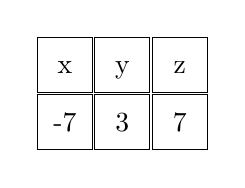
\begin{tikzpicture}
		\matrix (store) [table, text width=7mm, name=table]
			{ x & y & z \\
			 -7 & 3 & 7 \\ };
	\end{tikzpicture}
	\end{center}
	Here the variable
	$x$ holds the value $-7$, $y$ the value $3$ and $z$ $7$, thus:
	$s(x) = -7$, $s(y) = 3$, $s(z) = 7$.
	Furthermore $\text{dom}(s) = \{x,y,z\}$.
	\end{myexp}

	The \emph{Heap} is a formalisation of addressable memory which can be
	dynamically allocated by a program. It manages memory cells which contain
	integer values and are uniquely identified by a natural number as their
	address.
	\begin{mydef}[\emph{Heap}]
		A \emph{Heap} is a finite partial function
		$h:\mathbb{N} \rightharpoonup \textit{Integers}$
	\end{mydef}
	\begin{myexp}[\emph{Heap}]
	A possible state for a \emph{Heap} $h$.\\
	\begin{center}
	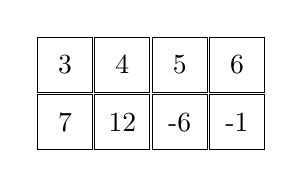
\begin{tikzpicture}
		\matrix (store) [table, text width=7mm, name=table]
			{ 3 &  4 &  5 &  6 \\
			  7 & 12 & -6 & -1 \\ };
	\end{tikzpicture}
	\end{center}
	\label{fig:heap}
	 Here the cell with address
	$3$ holds the value $7$, the cell with address $4$ the value 12,
	the cell with address $5$ the value -6 and the cell with address $6$ the
	value -1,
	thus: $h(3) = 7$, $h(4) = 12$, $h(5) = -6$, $h(6)=-1$.
	Furthermore $\text{dom}(h) = \{3,4,5,6\}$.
	\end{myexp}

	%semantik, wie man store Variablen interpretiert:
	Because the mapping of the program's variables is now formalised by the
	\emph{Store} an expression $E$ which is for example used in the
	\emph{Axiom of Assignment} in \emph{Hoare Calculus} needs interpretation.
	The \emph{Store} gives the syntactical objects of variables their values. Therefore
	the syntax $\llbracket E \rrbracket s$ will be used to refer to the expression
	$E$ where all variables are interpreted by the \emph{Store} $s$. Referring to
	the example of the \emph{Store} above the expression $x + y$ is evaluated to
	$\llbracket x + y \rrbracket s \equiv s(x) + s(y) = -7 + 3 = 4$. The same
	applies to boolean expressions $B$ which are evaluated over a \emph{Store}
	$s$ written as $\llbracket B \rrbracket s$. For example using the \emph{Store}
	$s$ from the example above $x + 7 > z$ is evaluated to
	${\llbracket x + 7 > z \rrbracket s} {\;\equiv s(x) + 7 > s(z)}
	 {\;\equiv -7 + 7 > 7} {\;\equiv  0 > 7} {\;\equiv \textit{false}}$.

	\subsection{Logical Operators}
	In order to use the model of \emph{Stores} and \emph{Heaps} the used logic
	has to be able to state properties of those.
	To this aim the logic is enriched with some expressions for which an intuition
	will be given initially and which will be then defined in terms of
	\emph{Heaps} and \emph{Stores} later on.

	Firstly, the "$\mapsto$ operator" is used to connect the address of one cell
	with its content. For example $5\mapsto 2$ states that the cell which is
	addressed by $5$ holds the value $2$ or more generally, $E\mapsto F$ states
	that the value of the cell which is addressed by the value of the expression
	$E$ is the value of the expression $F$.

	Secondly, the $\ast$-operator is used to connect two assertions which are
	given for two disjunctive parts of the current state of the \emph{Heap}.
	That means $P\ast Q$ for two assertions $P,Q$
	expresses that the allocated memory cells can be split into two independent
	parts where one satisfies $P$ and the other satisfies $Q$.

	Thirdly, the expression \textit{emp} is used to express that there are no cells
	in the \emph{Heap} allocated yet.

	Fourthly, the meaning of the $\forall$-operator slightly changes to its common
	interpretation because the
	\emph{Store} is used to map variables to values. Because the statement
	$\forall x.P$ for an assertion $P$ needs to be true for
	a \emph{Heap} and a \emph{Store} for every possible value $x$ can hold. But
	$x$ is evaluated through the \emph{Store} which means that the definition of
	$\forall$ is adjusted to take that into account. This applies in the same way
	to the $\exists$-operator.

	With this intuition in mind the definitions of the operator for \emph{Stores}
	and \emph{Heaps} follow naturally. For those
	assume that $s$ is a \emph{Store}, $h,h_1,h_2$ are \emph{Heaps}, $B$ is a
	boolean expression and $P$ is an assertion, and the syntax $s, h \models P$
	means that the assertion $P$ holds for the current state of the \emph{Store}
	$s$ and the \emph{Heap} $h$.
	\begin{mydef}[Logical Assertions]
		The semantic definitions for the \emph{logical assertions} are:\\
		\begin{center}
		\begin{tabular}{lll}
			$s, h \models E\mapsto F$ &iff &$\llbracket E\rrbracket s  = \textit{dom}(h) \text{ and }
			                               h(\llbracket E\rrbracket s) = \llbracket F\rrbracket s$ \\
			&&\\
			$s, h \models P\ast Q$ &iff &$\exists h_0,h_1.\;h_0\#h_1,\;h_0\bullet h_1=h,\;
			s,h_0 \models P \text{ and } s,h_1\models Q$\\
			&&\\
			$s, h \models\textit{emp}$ &iff  &$\textit{dom}(h) = \emptyset$\\
			&&\\
			$s, h \models B$ &iff &$\llbracket B\rrbracket s \equiv \textit{true}$\\
			&&\\
			$s, h \models \forall x.P$ &iff &$\forall v \in \textit{Integers}.(s|x\mapsto v),h \models P$\\
			&&\\
			$s, h \models \exists x.P$ &iff &$\exists v \in \textit{Integers}.(s|x\mapsto v),h \models P$\\
		\end{tabular}
		\end{center}
	\end{mydef}
	Note that for $E\mapsto F$ the \emph{Heap} consists of only one cell, but
	with $\ast$ more complex \emph{Heaps} can be described. For example for the
	\emph{Heap} $h$ and the \emph{Store} $s$ from the
	examples above applies $s, h \models y\mapsto 7\ast 4\mapsto 12
	\ast 5\mapsto x+1\ast 6\mapsto -1$.

	\subsection{Program Syntax}
	As mentioned in the introduction to \emph{Hoare Calculus} the formal language
	used to define programs lacks a syntax of accessing memory cells in the
	\emph{Heap}. In order to introduce such a syntax and connect it to the
	corresponding logical assertions further axioms are introduced below.

	First of all, there is no explicit way to state that a variable is used as
	reference to a memory cell. Rather every
	natural number can be interpreted as pointer. Therefore the syntax $[n]$ for
	$n\in\mathbb{N}$ is used as the content of the cell with address $n$.
	For example if for the current \emph{Heap} $h$ the following holds: $3\in\textit{dom}(h)$
	and $h(3) = 5$ then in the program the condition statement $([3] = 5)$ would evaluate to
	\textit{true}. For the definition of the new axioms one syntactical simplification
	is introduced as $E \mapsto -$ which is an abbrevation for
	$\exists y.E\mapsto y$. For the following definitions $E,F$ are integer
	expressions(expressions that are evaluated to an integer value by the
	programming language), $m$ is an integer and $x$ is a variable currently defined in
	the \emph{Store} $s$.
	\newcounter{AxiomIndex}
	\setcounter{AxiomIndex}{1}
	\begin{mydef}[Axioms of Referenced Access]
		The Hoare-triples\\
		\begin{center}
		\begin{tabular}{llll}
			\arabic{AxiomIndex}\stepcounter{AxiomIndex}&
			$\{ E \mapsto - \}$ &$[E] := F$ &$\{ E \mapsto F \}$\\
			&&&\\
			\arabic{AxiomIndex}\stepcounter{AxiomIndex}&
			$\{E \mapsto n \land \llbracket x\rrbracket s = m\}$ &
				$x := [E]$ &$\{\llbracket x \rrbracket s=n \land E[m/x]\mapsto n\}$\\
			&&&\\
			\arabic{AxiomIndex}\stepcounter{AxiomIndex}&
			$\{E \mapsto - \}$ &$\textit{dispose}(E)$ &$\{\textit{emp}\}$\\
			&&&\\
			\arabic{AxiomIndex}\stepcounter{AxiomIndex}&
			$\{\textit{emp}\}$ &$x := \textit{new}()$ &$\{x\mapsto -\}$\\
			&&\\
		\end{tabular}
		\end{center}
		are partially correct.
	\end{mydef}
	Note that new() returns a memory address which is not yet in the domain
	of the \emph{Heap} and in the second axiom the assignment
	of a value to $x$ can change the value of $E$. This is the reason
	for using the logical variable $m$ which persists through the assignment
	to replace occurences of $x$ in $E$. The definition of \textit{dispose} is
	taken from \cite{PermAcc}.

	In order to conclude the section about \emph{Separation Logic} the
	\emph{Frame Rule} is introduced. The \emph{Frame Rule} is used to reason
	locally about programs. This means for any subprogram it is only necessary
	to give assertions about the heap-cells which are actually used and modified
	in the subprogram. Therefore any other cell in the \emph{Heap} does not have
	effect on the subprogram. The \emph{Frame Rule} is presented as interference
	rule:
	\begin{mydef}[Frame Rule]
		For a program $C$ and assertions $P,Q,R$ holds:
		\begin{prooftree}
			\AxiomC{$\{P\}C\{Q\}$}
			\RightLabel{$\textit{modifies}(C)\cap\textit{free}(R) = \emptyset$}
			\UnaryInfC{$\{P\ast R\}C\{Q\ast R\}$}
		\end{prooftree}
	where $\textit{modifies}(C)$ is the set of variables modified by $C$ and
	$\textit{free}(R)$ the set of free variables in $R$.
	\end{mydef}
	These are the used rules and axioms for \emph{Separation Logic} in this paper.
	But as stated in \cite{freshlook} it is possible to work with other approaches
	to model the memory and mutable data structures therefore the presented
	axioms and rules are only a representative set.
	Following one small example will be examined:
	\begin{myexp}[Highest Value of Array]
		This example is a procedure which determines the highest value
		of an array. Because there is no defined syntax for an array it
		is expected to be a consecutive block of memory cells. The procedure
		takes a pointer to the first cell of the array and the length of the
		array. Firstly, a possible implementation is given, where \emph{skip}
		is the command that does nothing:
		\begin{lstlisting}[mathescape]
procedure maxValue($l$,$n$) {
	maxV := [l];
	m := 1;
	while(m < n) {
		if(maxV < [l + m]) {
			maxV := [l + m];
		} else {
			skip;
		}
		m := m + 1;
	}
}
		\end{lstlisting}
		Now in place reasoning is used to prove that \emph{maxV} will hold
		the maximal value of the array at the end of the procedure. For the
		programming lines comments are given which states the axiom or rule used to
		modify the assertions.
		\begin{lstlisting}[mathescape,tabsize=2,escapeinside={-<}{>-}]
-<\textcolor{green}{$\{l\mapsto v_1\ast l+1\mapsto v_2\ast\cdots\ast l+n-1\mapsto v_n\land\llbracket n\rrbracket s > 0\}$}>-
// the array needs to have at least one element
// and to be a consecutive block of memory cells
procedure maxValue($l$,$n$) {
-<\textcolor{green}{$\{l\mapsto v_1\ast l+1\mapsto v_2\ast\cdots\ast l+n-1\mapsto v_n\land\llbracket n\rrbracket s > 0\}$}>-
-<\textcolor{green}{$\therefore\{l\mapsto v_1\ast l+1\mapsto v_2\ast\cdots\ast l+n-1\mapsto v_n\land\llbracket n\rrbracket s>0 \land$}>-
-<\textcolor{green}{$\llbracket maxV \rrbracket s = \llbracket maxV \rrbracket s \land \llbracket m \rrbracket s = \llbracket m \rrbracket s\}$}>-
	maxV := [l]; // Axioms of Referenced Access
	m := 1; // Axiom of Assignment
	-<\textcolor{green}{$\{l\mapsto v_1\ast l+1\mapsto v_2\ast\cdots\ast l+n-1\mapsto v_n\land\llbracket n\rrbracket s>0 \land$}>-
	-<\textcolor{green}{$\llbracket maxV \rrbracket s = v_1 \land \llbracket m \rrbracket s = 1\}$}>-
	// loop invariant is: $m \leq n \land maxV = \max_{1\leq j\leq m}v_j$
	-<\textcolor{green}{$\therefore\{l\mapsto v_1\ast l+1\mapsto v_2\ast\cdots\ast l+n-1\mapsto v_n\land\llbracket n\rrbracket s>0 \land$}>-
	-<\textcolor{green}{$m \leq n \land \llbracket maxV\rrbracket s = \max_{1\leq j\leq m}v_j\}$}>-
	while(m < n) {
	-<\textcolor{green}{$\{l\mapsto v_1\ast l+1\mapsto v_2\ast\cdots\ast l+n-1\mapsto v_n\land\llbracket n\rrbracket s>0 \land$}>-
	-<\textcolor{green}{$m \leq n \land \llbracket maxV\rrbracket s = \max_{1\leq j\leq m}v_j\land \llbracket m \rrbracket s < \llbracket n \rrbracket s\}$}>-
		if(maxV < [l + m]) { // if-Rule
			-<\textcolor{green}{$\{l\mapsto v_1\ast l+1\mapsto v_2\ast\cdots\ast l+n-1\mapsto v_n\land\llbracket n\rrbracket s>0 \land$}>-
			-<\textcolor{green}{$\llbracket m\rrbracket s \leq \llbracket n\rrbracket s \land \llbracket maxV\rrbracket s = \max_{1\leq j\leq m}v_j$}>-
			-<\textcolor{green}{$\land \llbracket m \rrbracket s < \llbracket n \rrbracket s \land \llbracket maxV \rrbracket s < v_{m+1}\}$}>-
			-<\textcolor{green}{$\therefore\{l\mapsto v_1\ast l+1\mapsto v_2\ast\cdots\ast l+n-1\mapsto v_n\land\llbracket n\rrbracket s>0 \land$}>-
			-<\textcolor{green}{$\llbracket m\rrbracket s \leq \llbracket n\rrbracket s \land v_{m+1} = \max_{1\leq j\leq m + 1}v_j$}>-
			-<\textcolor{green}{$\land \llbracket m \rrbracket s < \llbracket n \rrbracket s \}$}>-
			maxV := [l + m]; // Axioms of Referenced Access
			-<\textcolor{green}{$\{l\mapsto v_1\ast l+1\mapsto v_2\ast\cdots\ast l+n-1\mapsto v_n\land\llbracket n\rrbracket s>0 \land$}>-
			-<\textcolor{green}{$\llbracket m\rrbracket s\leq\llbracket n\rrbracket s\land \llbracket maxV\rrbracket s = \max_{1\leq j\leq m + 1}v_j$}>-
			-<\textcolor{green}{$\land\llbracket m\rrbracket s<\llbracket n\rrbracket s\}$}>-
		} else {
			skip;
			-<\textcolor{green}{$\{l\mapsto v_1\ast l+1\mapsto v_2\ast\cdots\ast l+n-1\mapsto v_n\land\llbracket n\rrbracket s>0 \land$}>-
			-<\textcolor{green}{$\llbracket m\rrbracket s \leq \llbracket n\rrbracket s \land \llbracket maxV\rrbracket s = \max_{1\leq j\leq m}v_j$}>-
			-<\textcolor{green}{$\land \llbracket m \rrbracket s < \llbracket n \rrbracket s \land \llbracket maxV \rrbracket s \geq v_{m+1}\}$}>-
			-<\textcolor{green}{$\therefore\{l\mapsto v_1\ast l+1\mapsto v_2\ast\cdots\ast l+n-1\mapsto v_n\land\llbracket n\rrbracket s>0 \land$}>-
			-<\textcolor{green}{$\llbracket m\rrbracket s \leq \llbracket n\rrbracket s \land \llbracket maxV\rrbracket s = \max_{1\leq j\leq m + 1}v_j$}>-
			-<\textcolor{green}{$\land \llbracket m \rrbracket s < \llbracket n \rrbracket s \}$}>-
		}
		-<\textcolor{green}{$\{l\mapsto v_1\ast l+1\mapsto v_2\ast\cdots\ast l+n-1\mapsto v_n\land\llbracket n\rrbracket s>0 \land$}>-
		-<\textcolor{green}{$\llbracket m\rrbracket s \leq \llbracket n\rrbracket s \land \llbracket maxV\rrbracket s = \max_{1\leq j\leq m + 1}v_j$}>-
		-<\textcolor{green}{$\land \llbracket m \rrbracket s < \llbracket n \rrbracket s \}$}>-
		-<\textcolor{green}{$\therefore\{l\mapsto v_1\ast l+1\mapsto v_2\ast\cdots\ast l+n-1\mapsto v_n\land\llbracket n\rrbracket s>0 \land$}>-
		-<\textcolor{green}{$\llbracket m+1\rrbracket s \leq \llbracket n\rrbracket s \land \llbracket maxV\rrbracket s = \max_{1\leq j\leq m + 1}v_j\}$}>-
		m := m + 1; // Axiom of Assignment
		-<\textcolor{green}{$\{l\mapsto v_1\ast l+1\mapsto v_2\ast\cdots\ast l+n-1\mapsto v_n\land\llbracket n\rrbracket s>0 \land$}>-
		-<\textcolor{green}{$\llbracket m\rrbracket s \leq \llbracket n\rrbracket s \land \llbracket maxV\rrbracket s = \max_{1\leq j\leq m}v_j\}$}>-
	}
	-<\textcolor{green}{$\{l\mapsto v_1\ast l+1\mapsto v_2\ast\cdots\ast l+n-1\mapsto v_n\land\llbracket n\rrbracket s>0 \land$}>-
	-<\textcolor{green}{$\llbracket m\rrbracket s \leq \llbracket n\rrbracket s \land \llbracket maxV\rrbracket s = \max_{1\leq j\leq m}v_j$}>-
	-<\textcolor{green}{$\land \llbracket m\rrbracket s\geq \llbracket n\rrbracket s\}$}>-
	-<\textcolor{green}{$\therefore\{l\mapsto v_1\ast l+1\mapsto v_2\ast\cdots\ast l+n-1\mapsto v_n\land\llbracket n\rrbracket s>0 \land$}>-
	-<\textcolor{green}{$\llbracket m\rrbracket s = \llbracket n\rrbracket s \land \llbracket maxV\rrbracket s = \max_{1\leq j\leq m}v_j\}$}>-
	-<\textcolor{green}{$\therefore\{l\mapsto v_1\ast l+1\mapsto v_2\ast\cdots\ast l+n-1\mapsto v_n\land\llbracket n\rrbracket s>0 \land$}>-
	-<\textcolor{green}{$\land \llbracket maxV\rrbracket s = \max_{1\leq j\leq n}v_j\}$}>-
}
		\end{lstlisting}
	As this example shows it is a daunting task to reason about programs by hand.
	But the assertions above prove that the variable \emph{maxV}
	holds the highest value of the array, just as requested.
	\end{myexp}


%Section 3:
\section{Permission Accounting}
	%outline:
%	\begin{itemize}
%		%programming related:
%		\item read/write difference
%		\item mutual exclusion
%		%logic/proof related:
%		\item separation logic: conditional critical regions: CCR
%		\item fractional permissions
%		\item counting permissions
%		\item combine both approaches
%	\end{itemize}

	\emph{Separation Logic} as introduced above is used to reason about mutable data
	structures in the \emph{Heap} which is therefore separated into independent
	parts. This separation can be used to address concurrency by separating
	the \emph{Heap} and executing every concurrent program on its "own" part
	of the \emph{Heap}. Furthermore a system of permissions is introduced to
	share memory between concurrent threads as well as mechanisms to provide
	mutual-exclusive access on memory. 

	\subsection{Concurrency in \emph{Separation Logic}}
	This approach on concurrency in \emph{Separation Logic} is predominantly
	based on \cite{ConcurrencyInSepLogic} and \cite{PermAcc}.

	Concurrently executing programs which access the same memory, threaten to
	be \emph{racy}. This means that the values of variables or memory cells might not
	be only dependent on the commands of the programs but also from unintended
	access to shared memory by other programs. This may occur if two or more
	programs access shared memory at the same time, then the result of both
	operations depend on surrounding factors like for example the scheduler of
	the machine. \emph{Racy} programs are not easily reasoned about because it requires
	deep knowledge about the current state of the executing machine which might
	differ for every execution. Therefore it seems reasonable to have a guaranty that
	concurrent programs are not \emph{racy}, which is called \emph{race-free}.

	In order to access variables \emph{race-freely} from concurrent programs
	\cite{PermAcc} states that the variables
	need to be part of one of the following three groups of variables:
	Firstly, variables which are read and written exclusivly by one
	program. Secondly, variables which are accessed from concurrent programs but
	are only read. And thirdly, variables which are accessed from concurrent
	programs but where the write access is only allowed in a mutually-exclusive
	section of the program, i.e. a section which guarantees that in the
	meantime no other thread accesses those variables.

	In what follows a syntax for concurrent execution of programs is introduced as:
	\begin{mydef}[Concurrent Execution]
		For two programs $C_1,C_2$
		$$C_1\parallel C_2$$
		defines \emph{concurrent execution} of $C_1$ and $C_2$.
	\end{mydef}

	As stated above programs with variables read and written exclusivly by
	the program itself are race-free, also multiple programs which only
	\underline{read} from the same variables are race-free. This means
	race-freedom can be guaranteed for multiple concurrently executed programs
	if they only read from shared memory and if every modified variable is only
	accessed exclusively by one of the programs.

	\begin{mydef}[Concurrency Rule]
	Given $n$ programs $C_1,\dots,C_n$ with individual
	\emph{preconditions} $Q_1,\dots,Q_n$ and corresponding \emph{postconditions} $R_1,\dots,R_n$ where for
	every $i$: $\{Q_i\}C_i\{R_i\}$ is partially correct and race-free. If
	$\forall i,j \in \{1..n\}, i \neq j.(\text{free}(Q_i)\cup\text{free}(R_i))
	\cap \text{modifies}(C_j)  = \emptyset$ then
	$\{Q_1\ast\cdots\ast Q_n\}(C_1\parallel \cdots\parallel C_n)\{R_1\ast\cdots\ast R_n\}$
	is also partially correct and race-free. Stated as inference rule:
	\begin{prooftree}
	\AxiomC{$\{Q_1\}C_1\{R_1\}\cdots\{Q_n\}C_n\{R_n\}$}
	\UnaryInfC{$\{Q_1\ast\cdots\ast Q_n\}(C_1\parallel \cdots\parallel
		C_n)\{R_1\ast\cdots\ast R_n\}$}
	\end{prooftree}
	\end{mydef}
	\begin{myexp}[Concurrently executed Assignmend]
	Just to convay a basic intuition on using the concurrency rule
	the following example shows how three memory cells are assigned
	different values concurrently
	\begin{lstlisting}[mathescape]
x := new();
y := new();
z := new();
[x] := 5; $\parallel$ [y] := 7; $\parallel$ [z] := 13;
	\end{lstlisting}
	The program is obviously rather simple but it may help to examine an
	easy example first. Now assertions are added, and as well some comments
	to explain details:
	\begin{lstlisting}[mathescape, escapeinside={-<}{>-}]
-<\textcolor{green}{$\{\textit{emp}\}$}>-
x := new();  // Axioms of Referenced Access
-<\textcolor{green}{$\{x\mapsto -\}$}>-
-<\textcolor{green}{$\therefore\{x\mapsto - \ast \textit{emp}\}$}>-
// emp is the neutral element of the operator $\ast$ and can 
// therefore be added to any heap
y := new(); // Axioms of Referenced Access
-<\textcolor{green}{$\{x\mapsto - \ast y \mapsto -\}$}>-
// Note that new() is expected to return another value for $y$ than for $x$
// because the cell $x$ points to is already allocated, and therefore $x\mapsto -$
// and $y\mapsto -$ can be separated with $\ast$
-<\textcolor{green}{$\therefore\{x\mapsto - \ast y\mapsto - \ast \textit{emp}\}$}>-
z := new(); // Axioms of Referenced Access
-<\textcolor{green}{$\{x\mapsto - \ast y\mapsto - \ast z\mapsto -\}$}>-
[x] := 5; $\parallel$ [y] := 7; $\parallel$ [z] := 13;
-<\textcolor{green}{$\{x\mapsto 5 \ast y\mapsto 7 \ast z\mapsto 13\}$}>- // Concurrency Rule
	\end{lstlisting}
	Actually, the side conditions of the \emph{Concurrency Rule} needs to be
	checked to apply it. But this is omitted due to its simplicity.
	\end{myexp}

	But as stated above programs are also race-free if the access to a variable
	or shared memory is guaranteed to be mutual-exclusive. In order to provide
	such a mutual-exclusive access
	the formal language which is used in this paper to define programs, is
	extended with a mechanism of \emph{Conditional Critical Region(CCR)}. A
	\emph{CCR} is used to provide mutual-exclusive access to resources, namely
	variables and shared memory.
	Those resources can be collected in a set which is called a \emph{bundle}.
	For a \emph{bundle} $b$, a boolean expression $G$ and a program $C$ a
	\emph{CCR} is a command of the form:
	\begin{lstlisting}[mathescape]
with $b$
when $G$ do
	$C$
od
	\end{lstlisting}
	The idea is to provide mutual-exclusive access to all resources in the
	\emph{bundle} $b$ within $G$ and $C$. This means that the 
	resources in $b$ must not be accessed from outside the \emph{CCR},
	but can be accessed from inside with the guarantee that there is no
	other access at the same time from another program.

	A \emph{CCR} is handled in the following way:
	\begin{enumerate}
		\item the \emph{bundle} $b$ is aquired, i. e. an exclusive access
			on all items of the \emph{bundle} is guaranteed
		\item the condition $G$ is evaluated
		\item if $G$ is true, the program $C$ is executed and afterwards $b$ is
			released
		\item if $G$ is false, $b$ is released and the execution continues at step 1
	\end{enumerate}
	Having this in mind it is rather intuitive that this allows race-free sharing
	of resources, because of step 1. But to link this syntactical element to
	logical assertions, it is helpful to give another reading to the
	"$\mapsto$ operator": It can be understood as the permission to access the
	memory cell.
	And this right to access the memory cells of $b$ is only granted within the
	\emph{CCR}. Therefore to prove properties of a \emph{CCR} one needs an
	invariant $I_b$ for a \emph{bundle} $b$ which is only accessible within the
	\emph{CCR} and cannot be accessed from outside the \emph{CCR}. This invariant
	is used in a similar way as in the proofs for loops in \emph{Hoare Calculus},
	because if an invariant exists which all concurrent programs respect, this
	assertion can always be guaranteed. The following rule formalises that the
	variables of a \emph{bundle} can only be accessed within a \emph{CCR}:
	
	\begin{mydef}[CCR Rule]
		For a \emph{bundle} $b$, a boolean expression $G$, a program $C$,
		assertions $Q, R$ and an invariant $I_b$, the following inference rule
		holds regarding race-freedom and partial correctness:
	\begin{prooftree}
		\AxiomC{$\{(Q\ast I_b) \land G\} C \{R \ast I_b\}$}
		\UnaryInfC{$\{Q\}\text{with $b$ when $G$ do $C$ od}\{R\}$}
	\end{prooftree}
	\end{mydef}

\subsection{Abstract Permission Model}
	The abstraction of \emph{Permission Models} is mainly based on
	\cite{freshlook} and \cite{PermAcc}.

	As already mentioned the "$\mapsto$ operator" can be read as a permission to
	access a certain memory cell. In the following this reading is expanded to
	distinguish between read and write access to a cell. By now a memory cell can always
	be part of only one independent part of the \emph{Heap} which is separated
	from others by $\ast$. But a cell which is only read can be logically
	associated with multiple part of the \emph{Heap} where all parts of the 
	\emph{Heaps} need to agree on the value of the cell. This can be used to
	formulate assertions for programs which only need a read access on a
	cell. Obviously multiple possibilities to implement such a
	\emph{Permission Accounting} exist. But all of these implementations need to
	have certain properties. These properties are now defined and later on
	different possibilities of actually realising a permission model are
	introduced.

	A model which allows \emph{Permission Accounting} needs to manage permission
	associated with every access on cells of the \emph{Heap}. Therefore the
	definition of \emph{Heaps} slightly adapts to
	\begin{mydef}[Heap]
		For a set of addresses $L$, a set of values $V$ and a set of
		permissions $M$ a \emph{Heap} is defined as partial function
		$$h: L \rightharpoonup (V\times M)$$
	\end{mydef}
	\noindent
	Note that the set of addresses and the set of values are not explicitly
	defined. For all \emph{Heaps} above always applied $L = \mathbb{N}$ and
	$V = \textit{Integers}$. But although addressable memory cells are very
	intuitive, the dynamically allocatable memory of programs might be
	represented differently. For example with \emph{Petri Nets} \cite{seplogproof}.

	Regarding the set of permissions $M$ the intuitive idea is that
	exactly one \emph{source permission} exists which grants full access rights
	on a cell including read and write permission as well as the permission to
	dispose the cell. From a \emph{source permission} multiple read permissions
	can be derived. Deriving a read permission from a \emph{source permission}
	causes the \emph{source permission} to loose the right of writing and
	disposing the cell, it becomes a read permission as well to avoid \emph{racy}
	behaviour. A \emph{source permission} can always be regained by recombining
	all permissions of a cell.
	This is mathematically represented by a binary operator for the elements of
	$M$ which adds permissions together and can be used to
	define splitting of a permission. This operator is commutative, because the
	order of how permissions are recombined does not matter. There is no neutral
	element to this operator because the not granted permission is always
	implicitly stated by not mentioning a cell in an assertion.
	Additionally, certain elements can not be combined, for example two
	\emph{source permissions} for the same cell. Mathematically speaking:
	\begin{mydef}[Permission]
		A set of permissions $M$ is equipped with a partial commutative
		semigroup structure with the binary operator $\oplus$.
	\end{mydef}
	The \emph{source permission} needs to be unique and can not be expanded
	further because it already is the maximal permission. Futhermore every
	permission can be recombined to a \emph{source permission} again:
	\begin{mydef}[Source permission]
		In a set of permissions $M$ exists exactly one $m_W$ with:
		$$\forall m\in M.m_W\oplus m\text{ is undefined}$$
		$$\forall m\in M\setminus \{m_W\} \exists m'. m \oplus m' = m_W$$
	\end{mydef}
	This permission model is now connected to cells by expanding the operator
	$\oplus$ to the set $(V\times M)$ as
	$$(v,m)\oplus(v',m') =
		\begin{cases}
			(v,m\oplus m') &\text{ if $v=v'$ and $m\oplus m'$ \textit{defined}}\\
			\text{undefined} &\text{ otherwise}\\
		\end{cases}
	$$
	Note that two cells can only be combined if they agree on the value $v$.

	Correspondingly, the operator is also applied to \emph{Heaps} but to fit
	the definitions above it is named $\ast$:
	\begin{mydef}[Separation of Heaps]
		If for two \emph{Heaps} $h,h'$ for each $l\in \textit{dom}(h)\cap\textit{dom}(h')$ $h(l)\oplus h'(l)$
		is defined the \emph{Separation} of those(written as $h\ast h'$)
		is defined as:
		$$(h\ast h')(l) =
			\begin{cases}
				h(l) &\text{ if $h'(l)$ undefined}\\
				h'(l)&\text{ if $h(l)$ undefined}\\
				h(l) \oplus h'(l) &\text{ otherwise}\\
			\end{cases}
		$$
	\end{mydef}

	This abstraction of \emph{Permission Accounting} needs to be connected to
	the programming syntax. For convenience the following syntax will be used
	for a program $C$, \emph{Stores} $s,s'$ and \emph{Heaps} $h,h'$:
	$C,s,h \leadsto s', h'$. This means the command $C$ executed on a
	\emph{Heap} $h$ and a \emph{Store} $s$ leads to a \emph{Heap} $h'$ and a
	\emph{Store} $s'$. Using this new syntax the commands of the programming
	language can be defined as follows:
	\begin{mydef}[Semantics of commands]
	For a \emph{Store} $s$, a set of values $V$, a set of addresses $L$, a
	set of permissions $M$ with a maximum permission of $m_W$, a \emph{Heap}
	$h:L \rightharpoonup (V\times M)$, integer expressions $E,E'$ and $v\in V$,
	$l\in L$,$x\in \textit{Vars}$ the definition of the commands are:\\
		\begin{center}
		\begin{prooftree}
		\AxiomC{$\llbracket E \rrbracket s = v$}
		\UnaryInfC{$x:=E,\; s,h \leadsto (s|x\mapsto v),h$}
		\end{prooftree}
		\end{center}
		\begin{center}
		\begin{prooftree}
		\AxiomC{$\llbracket E'\rrbracket s = l$}
		\AxiomC{$\llbracket E \rrbracket s = v$}
		\AxiomC{$h(l) = (-,m_W)$}
		\TrinaryInfC{$[E'] := E,\; s,h \leadsto s,(h|l\mapsto(v,m_W))$}
		\end{prooftree}
		\end{center}
		\begin{center}
		\begin{prooftree}
		\AxiomC{$\llbracket E'\rrbracket s = l$}
		\AxiomC{$h(l) = (v, m)$}
		\BinaryInfC{$x:=[E'],\; s,h \leadsto (s|x\mapsto v),h$}
		\end{prooftree}
		\end{center}
		\begin{center}
		\begin{prooftree}
		\AxiomC{$l \in L \setminus \text{dom}(h)$}
		\AxiomC{$\llbracket E \rrbracket s = v$}
		\BinaryInfC{$x:=\text{new}(E),\; s,h \leadsto (s|x\mapsto l),(h|l\mapsto(v,m_W))$}
		\end{prooftree}
		\end{center}
		\begin{center}
		\begin{prooftree}
		\AxiomC{$\llbracket E'\rrbracket s = l$}
		\AxiomC{$h(l) = (v,m_W)$}
		\BinaryInfC{$\text{dispose } E',\; s,h \leadsto s, (h\setminus{\{(l,v)\}})$}
		\end{prooftree}
		\end{center}
	\end{mydef}
	\noindent
	Note that these are the definitions of the commands as above with enforced
	permissions. A \emph{source permission} is necessary for changing the content
	of and disposing a cell. Allocating a memory cell initially grants a
	\emph{source permission}. Also this semantics are restricted to the
	sequential execution of the programs.

	These semantics of commands yield the following axiomatic Hoare-triples,
	where the "$\mapsto$ operator" is decorated with a permission $z$ as
	$\xmapsto{z}$:
	\begin{mydef}[Axioms for Regulated Heap Access]
	For an assertion $P$, a variable $x$, value expressions $E, E'$, which are
	expressions that can be evaluated to a value from the value-set $V$, values
	$v, n$, a permission $m$, a \emph{source permission} $m_W$ and a
	\emph{Store} $s$ the axioms for a permission model $M$ are:\\
	\begin{center}
	\begin{tabular}{p{4cm}p{3cm}p{5cm}}
		$\{P[E/x]\}$ & $x:=E$ & $\{P\}$ \\
		$\{E\xmapsto{m_W}-\}$ & $[E'] := E$ & $\{E'\xmapsto{m_W}E\}$ \\
		$\{E\xmapsto{m} n \land \llbracket x\rrbracket s =v\}$ & $x:=[E]$ & $\{E[v/x]\xmapsto{m}n\land\llbracket x\rrbracket s = n\}$\\
		$\{\textit{emp}\}$ & $x:=\textit{new}()$ & $\{x \xmapsto{m_W} -\}$\\
		$\{E\xmapsto{m_W}\}$ & $\textit{dispose}(E)$ & $\{\textit{emp}\}$\\
	\end{tabular}
	\end{center}
	\end{mydef}

	\subsection{Permission Models}
	The different \emph{Permissions Models} are defined in \cite{freshlook} and
	\cite{PermAcc}.

	An example for a model of \emph{Permission Accounting} is the model of
	\emph{Fractional Permissions}. The intuitive idea of \emph{Fractional Permissions}
	is that $1$ is the \emph{source permission} and every permission can be split
	into fractions to grant read permissions. Every permission
	$z \in (0,1)\cap\mathbb{Q}$ is a read permission which can be split further.
	Now, $\oplus_\text{FP}$ needs to be defined but this is rather
	straightforward as:
	\begin{mydef}[Combining Fractional Permissions]
		For two permissions $z,z' \in (0,1]\cap\mathbb{Q}$ the combination
		$z \oplus_\text{FP} z'$ is defined as:
		$$z \oplus_\text{FP} z' =
			\begin{cases}
				\text{undefined} & \text{ if $z + z' > 1$} \\
				z + z' & \text{ otherwise} \\
			\end{cases}
		$$
	\end{mydef}
	The formal model for $(M, m_W, \oplus)$ is
	$((0,1]\cap\mathbb{Q},1,\oplus_\text{FP})$.

	Another model for \emph{Permission Accounting} is the model of
	\emph{Counting Permissions}. Here the \emph{source permission} gives away
	tokens of read permissions and counts how many of these tokens are given
	away. The \emph{source permission} is $0$. Read permissions are indicated
	by negative numbers and with every derived read permission the token counter
	is incremented for the \emph{source permission} which just means that the
	permission is incremented by $1$. This leads to a special role of the
	\emph{source permission} because it is the only permission indicated by
	a positive number(or $0$). It can be understood as a central instance which
	gives away read accesses, where for \emph{Fractional Permissions} are a
	decentralised approach because every split produces two homogen
	tokens. Formally \emph{Counting Permissions} are
	$(\mathbb{Z},0,\oplus_\text{CP})$ with
	$$z \oplus_\text{CP} z' =
		\begin{cases}
			\text{undefined} & \text{ if $z \geq 0$ and $z' \geq 0$}\\
			\text{undefined} & \text{ if ($z\geq 0$ or  $z' \geq 0$) and $z + z' < 0$}\\
			z + z'           & \text{ otherwise}
		\end{cases}
	$$

	In \cite{freshlook} other models for \emph{Permission Accounting} are
	mentioned like the \emph{Boolean Share Model} which models how
	\emph{Separation Logic} was introduced above without
	\emph{Permission Accounting}.

	\emph{Permission Accounting} is used to restrict access to memory cells.
	A restricted access to a memory cell, for example a read access can be
	given to a program. And every command of the program must not change
	the value of the memory cell. The property that a command does not change
	the value of a memory cell is called \emph{Passivity}:
	\begin{myprop}[Passivity]
		A command $C$ shows \emph{Passivity} on a cell if it has access to
		a cell but does not change it.
	\end{myprop}
	\begin{mylem}[Passivity of cells with read permissions]
		If a command $C$ has only read access to a memory cell, it shows
		\emph{Passivity} on that cell.
	\end{mylem}
	\begin{myproof}[Passivity of cells with read permissions]
		Let $C$ be a program, $l$ an address, $v,v'$ values and $z,z'$
		permissions with $z\neq m_W$, $z'\neq m_W$, $z \oplus z' = m_W$,
		$v \neq v'$. And for $C$ two possibilities can be distinguished:
		Firstly, $C$ is a sequential program. In that case \emph{Termination
		Monoticity} (formally introduced in \ref{sec:soundness}) is given,
		which means if $C$ terminates in a \emph{Heap} $h$ it also terminates
		in a \emph{Heap} $h\ast h'$ for $h'$ is a compatible \emph{Heap}.
		Assume
		$$\{l\xmapsto{z}v\}C\{l\xmapsto{z}v'\}$$
		is a partially correct and terminating Hoare-triple. With the
		\emph{Frame Rule} follows
		$$\{l\xmapsto{z}v \ast l\xmapsto{z'}v\}C\{l\xmapsto{z}v' \ast l\xmapsto{z'} v\}$$
		Where \emph{Termination Monoticity} states that this Hoare-triple terminates
		and the \emph{Frame Rule} states that this Hoare-triple is partially correct.
		But the \emph{postcondition} is obviously false, and therefore there is a
		contradiction, which means that $C$ can not change the value of the
		memory cell with address $l$. The memory cell shows \emph{Passivity}.

		Secondly, $C$ is concurrently executed program, which means $C$ might aquire
		further access permissions by using permissions from a \emph{bundle}
		$b$. This case is dealt with exemplatory, but the proof can be
		accordingly generalised:
		For the \emph{bundle} $b$ an invariant $I_b \equiv l\xmapsto{z'}-$ exists
		and $C \equiv \text{with }b\text{ when true do } [l] := v' \text{ od}$.
		Using the \emph{CCR Rule} one can show that:
		$$\{l\xmapsto{z}v\}C\{l\xmapsto{z}v'\}$$
		by the following proof:

		\begin{lstlisting}[mathescape]
$\{l\xmapsto{z}v\}$
with $b$ when true do
	$\{(l\xmapsto{z}v\ast l\xmapsto{z'}-) \land true\}$
	$\therefore\{l\xmapsto{m_W}v\}$
	$[l] := v';$
	$\{l\xmapsto{m_W}v'\}$
	$\therefore\{l\xmapsto{z}v'\ast l\xmapsto{z'}-\}$
od
$\{l\xmapsto{z}v'\}$
		\end{lstlisting}

		With the \emph{Frame Rule} it is possible to prove the  Hoare-triple:
		$$\{l\xmapsto{z}v\ast l\xmapsto{z'}v\}C\{l\xmapsto{z}v'\ast l\xmapsto{z'}v\}$$
		Now if $C$ is part of a set of concurrently executed programs as:
		$C_1,\dots,C_n$ with $\exists j\in \{1,\dots,n\}.C_j = C$. Let $Q_1,\dots,Q_n$
		be the according \emph{preconditions} and $R_1,\dots,R_n$ the \emph{postconditions}.
		The \emph{Concurrency Rule} would lead for $(C_1\parallel\cdots\parallel C_n)$
		to a \emph{precondition} with
		$\{\cdots\ast I_b \ast l\xmapsto{z}v \ast l\xmapsto{z'}v \ast\cdots\}$. This
		\emph{precondition} is not satisfyable because such a \emph{Heap} does not
		exist. Therefore $C$ can not be part of a concurrent execution but this
		was assumed, which means for a read permission \emph{Passivity} on the cell
		is guaranteed.
	\end{myproof}

	\subsection{Soundness and race-freedom}
	\label{sec:soundness}
	After having introduced \emph{Separation Logic} and
	\emph{Permission Accounting} as logical tools to reason about programs which
	can be executed concurrently, share memory between each other and access
	dynamically allocated memory, a proof for the soundness of the introduced
	rules and the race-freedom of the approach of \emph{Permission Accounting}
	would justify these approaches. This proof is given in \cite{seplogproof}
	and due to its complexity it can not be given here.
	Instead to convay an intuition on how to prove properties for
	\emph{Separation Logic} a few definitions regarding soundness of rules for
	sequentially executed programs which are based on \cite{sembasis} are
	introduced and exemplatory the \emph{Frame Rule} is examined.

	To examine formally the execution of a program it is understood as sequence
	of configurations. Configurations are current state of a machine, which is
	the state of the \emph{Heap} $h$, the state of the \emph{Store} $s$ and
	potentially a sequence of commands (a program) $C$. A configuration $(s, h)$
	where no more commands exist to be executed is called \emph{terminal}. A non
	\emph{terminal} configuration is a triple $(C, s, h)$. On the set of
	configurations the relation $\leadsto$ which was already utilized
	above for defining the semantics of the commands in \emph{Permission
	Accounting} is defined as the change of the configuration based on the
	executed command. In the previous definitions a program $C$ was expected to
	be well defined which means it does not access memory cells which are not
	allocated but now the set of configurations can be extended with a
	\textit{fault} state. The \textit{fault} state is reached if a memory cell
	not present in the \emph{Heap} $h$ is accessed. To get an intuition on
	configurations and $\leadsto$ a few relations are given:
	\begin{mydef}[Configuration Transitions]
	For a \emph{Heap} $h$, a \emph{Store} $s$, an integer expression $E$, a
	boolean expression $B$ and programs $C, C'$ the following relations on
	configurations are defined:
	\begin{enumerate}
	\item \begin{prooftree}
			\AxiomC{$\llbracket E \rrbracket s \notin \textit{dom}(h)$}
			\UnaryInfC{($x := [E],s,h)\leadsto \textit{fault}$}
			\end{prooftree}
	\item \begin{prooftree}
			\AxiomC{$\llbracket B \rrbracket s \equiv \textit{true}$}
			\UnaryInfC{(while $B$ do $C$ od, $s, h)\leadsto$(($C$; while $B$ do $C$ od), $s$, $h)$}
			\end{prooftree}
	\item \begin{prooftree}
			\AxiomC{$\llbracket B \rrbracket s \equiv \textit{false}$}
			\UnaryInfC{(if $B$ then $C$ else $C'$, $s,h)\leadsto (C', s, h)$}
			\end{prooftree}
	\end{enumerate}
	\end{mydef}

	The relation $\textit{Conf} \leadsto^\ast \textit{Conf'}$ states that
	there is a $\leadsto$-sequence of configurations from \textit{Conf} to
	\textit{Conf'}.
	In the following a configuration is called \emph{safe} if the execution from
	this configuration does not lead to a fault state.
	\begin{mydef}[Safety]
		A configuration $(C,s,h)$ is \emph{safe} if $(C,s,h)$ $\slashed{\leadsto}^\ast$ \textit{fault}.
	\end{mydef}
	This can be used to expand partial correctness to grand safety as well:
	\begin{mydef}[Partial Correctness with Safety]
		The Hoare-triple $\{P\}C\{R\}$ for a \emph{precondition} $P$, a
		\emph{postcondition} $R$ and a program $C$ is \emph{partially correct}
		if for all \emph{Stores} $s$ and \emph{Heaps} $h$ applies:
		if $s,\;h\models P$ then
			$(C,s,h)$ is safe, and if $(C,s,h)\leadsto^\ast (s',h')$ for a
			\emph{Store} $s'$ and a \emph{Heap} $h'$ then $s',\;h'\models R$.
	\end{mydef}
	As already mentioned programs exist which do not terminate. Such programs
	have an infinite $\leadsto$-sequence from their starting configuration.
	All programs which terminate for every state and which are partially correct
	are called totally correct:
	\begin{mydef}[Total Correctness]
		The Hoare-triple $\{P\}C\{R\}$ for a \emph{precondition} $P$, a
		\emph{postcondition} $R$ and a program $C$ is \emph{totally correct}
		if for all \emph{Stores} $s$ and \emph{Heaps} $h$ applies:
		if $s,\;h\models P$ then there is no infinite $\leadsto$-sequence
		starting from $(C,s,h)$ and if $(C,s,h) \leadsto (s',h')$ for
		a \emph{Store} $s'$ and a \emph{Heap} $h'$ then $(s',h')\models R$.
	\end{mydef}
	In order to prove the \emph{Frame Rule} sound for partial and total
	correctness it is essential to prove the locality of commands. Locality
	is the property that commands executed on one part of the \emph{Heap}
	do not affect any other part of the \emph{Heap} and that the behaviour of
	the command is not affected by any other part of the \emph{Heap}. This
	regards safety as well as termination of programs. Formally formulated
	as the following properties:
	\begin{myprop}[Safety Monotonicity]
		For a program $C$, a \emph{Store} $s$ and \emph{Heaps} $h,h'$:
		If $(C,s,h)$ is safe and $h\#h'$, then $(C,s,h\ast h')$ is safe.
	\end{myprop}
	\begin{myprop}[Termination Monotonicity]
		For a program $C$, a \emph{Store} $s$ and \emph{Heaps} $h,h'$:
		If there is no infinite sequence of configurations starting from
		$(C,s,h)$ and $h\#h'$, then there is no infinite sequence of
		configurations starting from $(C,s,h\ast h')$.
	\end{myprop}
	\begin{myprop}[Frame Property]
		For a program $C$, \emph{Stores} $s,s'$, \emph{Heaps} $h_0,h_1,h'$:
		If $(C,s,h_0)$ is safe and $(C,s,h_0\ast h_1) \leadsto^\ast (s',h')$
		then a \emph{Heap} $h_0'$ exists with $(C,s,h_0)\leadsto^\ast (s',h_0')$
		and $h' = h_0'\ast h_1$.
	\end{myprop}
	These properties are sufficient to prove the \emph{Frame Rule} sound by the
	following argument:
	\begin{mylem}[Soundness of the \emph{Frame Rule}]
		From \emph{Safety Monotonicity}, \emph{Termination Monotonicity} and
		the \emph{Frame Property} follows the soundness of the \emph{Frame Rule}
		for partial and total correctness.
	\end{mylem}
	\begin{myproof}
		Suppose $\{P\}C\{Q\}$ is a totally correct Hoare-triple. This means
		that for any \emph{Heap} $h_P$ and \emph{Store} $s$ with $(s,h_P)\models P$:
		$(C,s,h_P)\leadsto^\ast (s',h')$ gives us $(s',h')\models Q$. Let $s$
		be a \emph{Store}.
		Now let $h_R$ be any \emph{Heap} with $(s,h_R)\models R$. And $h_P$ any
		\emph{Heap} with $(s,h_P)\models P$. Because $(C,s,h_P)$ is safe it follows
		from \emph{Safety Monoticity} that $(C,s,h_P\ast h_R)$ is safe.
		\emph{Termination Monoticity} gives the existence of a \emph{Heap} $h$ with
		$(C,s,h_P\ast h_R) \leadsto^\ast (s',h)$. And for this \emph{Frame Property}
		yields $h_P'$ with $h_P'\ast h_R = h$ and $(C,s,h_P)\leadsto^\ast (s',h_P')$.
		Because $\{P\}C\{Q\}$ is totally correct and $(C,s,h_P)\leadsto^\ast (s',h_P')$
		it follows that $(s',h_P')\models Q$. Because of the side condition of the
		\emph{Frame Rule} the \emph{Stores} $s, s'$ agree on the values of every
		variable free in $R$. This means because $(s,h_R)\models R$ that $(s',h_R)\models R$.
		This gives $(s',h)\models Q\ast R$. Therefore the \emph{Frame Rule} is sound
		for partial and total correctness.
	\end{myproof}
	This means if the properties of \emph{Termination Monoticity},
	\emph{Safety Monoticity} and \emph{Frame Propery} can be proven for
	\emph{Heaps} build from \emph{Permission Accounting} the soundness of the
	\emph{Frame Rule} is given. As \cite{PermAcc} states the condition
	$$\forall m\in M. m_W\oplus m \text{ is undefined}$$
	ensures \emph{Frame Property} and \emph{Safety Monoticity}. This can be
	shown by the following arguments:
	\begin{myproof}[Frame Property of \emph{Heaps} with \emph{Permission Accounting}]
		Let the premisses of the \emph{Frame Property} hold. In the following
		$h, h_0, h_1, h_0'$ refers to \emph{Heaps} and $s$ to a \emph{Store}.

		For $[E'] := E$: Because $([E'],s,h_0)$ is safe by assumption, for a value $v$:
		$h_0(\llbracket E'\rrbracket s) = (v,m_W)$. This means that for $h_1$
		holds $\llbracket E'\rrbracket s \notin \textit{dom}(h_1)$ and therefore
		$[E'] := E$ does not affect $h_1$. With $h_0' = (h_0|\llbracket E'\rrbracket s = E)$
		gives $([E'] = E,s,h_0)\leadsto^\ast s', h_0'$ and $h' = h_0'\ast h_1$.

		For $\textit{dispose}(E)$: Let $l = \llbracket E \rrbracket s$. Because
		$(\textit{dispose}(E),s,h_0)$ is safe, a value $v$ exists with 
		$h_0(l) = (v, m_W)$. Therefore $l \notin \textit{dom}(h_1)$ and for
		$h_0'$ is the \emph{Heap} for which $h_0 = h_0' \ast l\mapsto v$ follows
		$(\textit{dispose}(E),s,h_0)\leadsto^\ast s', h_0'$ and $h' = h_0'\ast h_1$.

		For $x := [E]$: Let $l = \llbracket E \rrbracket s$ and because of the
		Safety of $(x:=[E],s,h_0)$ follows $l\in\textit{dom}(h_0)$ and with
		$h_0' = h_0$ the \emph{Frame Property} follows immediatly.

		For $\text{\emph{if }}B\text{\emph{ then }} C\text{\emph{ else }} C'$,
		$\text{\emph{while }}B\text{\emph{ do }} C \text{\emph{ od}}$, $C_1;C_2$:
		Consider a variant of \emph{Frame Property} as $(C,s,h_0)$ is
		safe and $(C,s,h_0\ast h_1) \leadsto^\ast (C',s',h')$ then there is a
		\emph{Heap} $h_0'$ with $(C,s,h_0)\leadsto^\ast (C',s',h_0)$ and $h'=h_0'\ast h_1$.
		Now the proof works with induction by the derivation steps for \emph{while}
		and \emph{if} and \emph{;} :
		Let $(\text{\emph{while }} B \text{\emph{ do }} C \text{\emph{ od}},s,h_0)$
		be safe and $(\text{\emph{while }} B \text{\emph{ do }} C \text{\emph{ od}},s,h_0)
		\leadsto^\ast(C',s',h')$. If $B$ is false this is one of the atomic cases
		for $(C, s, h_0)$, thus, $B$ is true:
		$(\text{\emph{while }} B \text{\emph{ do }} C \text{\emph{ od}},s,h_0)\leadsto
		 (C;\text{\emph{while }} B \text{\emph{ do }} C \text{\emph{ od}},s,h_0)$
		 and with the induction hypothesis for this deriveration \emph{Frame Property}
		 or its variant is already shown. This can be executed
		 analogically for \emph{if} and \emph{;}.
	\end{myproof}

	\begin{myproof}[Safety Monoticity of \emph{Heaps} with \emph{Permission Accounting}]
		If the configuration $(C,\;s,\;h)$ is safe there are two possiblities for
		every $l\in\textit{dom}(h)$:
		Firstly, the cell with address $l$ is only read. Then this right can not
		be taken away by adding another \emph{Heap} $h'$. This means $(C,s,h\ast h')$
		is safe as well.
		Secondly, the cell with address $l$ is written, which means that for a
		value $v$: $h(l) = (v, m_W)$ but this implies that for every \emph{Heap}
		$h'$ for which $h\ast h'$ is defined, holds: $l \notin\textit{dom}(h')$.
		Therefore $(C,s,h\ast h')$ is safe.
	\end{myproof}
	The proof of \emph{Termination Monoticity} works analogically to the proof
	of \emph{Safety Monoticity}.
	In conclusion the \emph{Frame Rule} is sound for \emph{Separation Logic} with
	\emph{Permission Accounting} for sequential programs.
	For a complete proof of soundness and race-freedom of concurrent programs
	in \emph{Separation Logic} with \emph{Permission Accounting} see \cite{seplogproof}.



%Section 4:
\section{Conclusion}
%	\begin{itemize}
%		\item way to reason about heaps
%		\item way to resourcing
%		\item basis for tool assisted proofs
%	\end{itemize}
	In conclusion, \emph{Separation Logic} was introduced as a tool to reason
	about mutable data structures in the \emph{Heap}. Therefore the syntax and
	semantics of the logic were introduced. To work with concurrently executed
	programs the fundamentals of sharing memory are introduced. Furthermore,
	\emph{Permission Accounting} was defined to grant different permissions on
	memory cells and the \emph{Passivity} of programs on memory cells for which
	only read permission is given was proven. As mentioned the soundness and
	race-freedom of this approach of \emph{Permission Accounting} are proven in
	\cite{seplogproof}. This approach leads to interesting further ideas.
	It is possible to adapt \emph{Permission Accounting} for the use in the
	\emph{Store} \cite{storeperm}. Furthermore, the introduced abstraction of
	the models for \emph{Permission Accounting} can be used to develop other
	models which include other useful properties. In \cite{freshlook} for example
	the property of \emph{Splittability} is introduced which states that a
	permission can be infinitly splitted. As stated in \cite{PermAcc}
	it is desirable to expand the term \emph{ressources} which can be shared
	between concurrent programs to fit everything a program can manage(e. g.,
	the used space, the processing time,\dots). And also, that the specification
	of every program has to explicitly state which ressources are required. And
	of course reasoning about programs is always interesting for computer aided
	verification\footnote{smallfoot - a verification tool, based on
	\emph{Separation Logic}; see http://www0.cs.ucl.ac.uk/staff/p.ohearn/smallfoot/}
	\cite{freshlook}.


\bibliography{./literature}
\bibliographystyle{abbrv}
\end{document}
